\documentclass[10pt,twocolumn,letterpaper]{article}

\usepackage{cite}
\usepackage{caption}
\usepackage{underscore}
\usepackage{cvpr}
\usepackage{times}
\usepackage{epsfig}
\usepackage{graphicx}
\usepackage{amsmath}
\usepackage{amssymb}
\usepackage[utf8]{inputenc}
\usepackage[T1]{fontenc}
\usepackage{lmodern} % load a font with all the characters

% Include other packages here, before hyperref.

% If you comment hyperref and then uncomment it, you should delete
% egpaper.aux before re-running latex.  (Or just hit 'q' on the first latex
% run, let it finish, and you should be clear).
\usepackage[breaklinks=true,bookmarks=false]{hyperref}

\cvprfinalcopy % *** Uncomment this line for the final submission

\def\cvprPaperID{****} % *** Enter the CVPR Paper ID here
\def\httilde{\mbox{\tt\raisebox{-.5ex}{\symbol{126}}}}

% Pages are numbered in submission mode, and unnumbered in camera-ready
%\ifcvprfinal\pagestyle{empty}\fi
\setcounter{page}{1}
\begin{document}

%%%%%%%%% TITLE
\title{Laboratorio 6: Clasificación por textones}

\author{Rafael Cuperman Coifman\\
Universidad de los Andes\\
Bogotá, Colombia\\
{\tt\small r.cuperman675@uniandes.edu.co}
% For a paper whose authors are all at the same institution,
% omit the following lines up until the closing ``}''.
% Additional authors and addresses can be added with ``\and'',
% just like the second author.
% To save space, use either the email address or home page, not both
}

\maketitle
%\thispagestyle{empty}

%%%%%%%%% ABSTRACT
\begin{abstract}
 En este experimento se construyen dos diferentes clasificadores para abordar el problema de reconocimiento de imágenes de acuerdo a sus texturas. Las imágenes son representadas mediante histogramas de textones variando el número de bins (textones). Se construye un modelo de clasificación mediante Nearest Neighbour con kernel de intersección y otro mediante Random Forest. El número de imágenes de entrenamiento, de textones y de árboles de decisión es variado para evaluar los desempeños de acuerdo a estos parámetros. Los resultados son presentados como matrices de confusión sobre imágenes de prueba junto con el error porcentual de clasificación en ellos para cada modelo creado. Se concluye que el método de Random Forest es más eficiente, en desempeño y tiempo, para la resolución de este problema bajo la base de datos \textit{Texture Database}, del grupo Ponce.
\end{abstract}

%%%%%%%%% BODY TEXT
%-------------------------------------------------------------------------
\section{Introducción}
Cuando se tienen varias categorías semánticas de imágenes que son difícilmente diferenciables de acuerdo a los colores presentes, una posibilidad para poder clasificarlas y reconocerlas es representarlas de acuerdo a las texturas que poseen. Si bien la textura no es una propiedad que trae una imagen en su representación matricial (como es el caso de los colores, donde cada píxel tiene asociado tres valores que determinan explícitamente el color de este), es una característica determinante en una figura. A diferencia del color, la textura es una característica no local, lo cual quiere decir que no tiene sentido hablar de la textura de un píxel aislado, sino de un grupo de píxeles sobre la imagen. Esto se debe a que las texturas se definen como patrones, por lo que es necesario analizar varios píxeles para detectarlas. La representación de las imágenes en este caso es, entonces, mediante textones.

En este experimento se entrenaron dos tipos clasificadores supervisados distintos para clasificar imágenes de acuerdo a sus texturas según la base de datos utilizada, y se compararon sus desempeños en términos de tiempo y eficiencia en clasificación.

\subsection{Base de datos \cite{Base}} 
La base de datos utilizada se llama \textit{Texture Database} y es del grupo Ponce, el grupo de Vision Artifical y Robótica de la Universidad de Illinois en Urbana-Champaign. Esta base de datos de imágenes con texturas tiene 25 clases, donde cada una de ellas tiene 40 imágenes. Todas las imágenes se encuentran en escala de gris en formato .jpg y son de \(640\times480\) píxeles. Las imágenes encontradas en esta base de datos corresponden a acercamientos a texturas naturales o sintéticas, como por ejemplo troncos de árboles, telas, madera, ladrillos y pelo, entre otros en diferentes orientaciones y perspectivas.La base de datos se dividió en dos: 30 imágenes por categoría para entrenamiento y las 10 restantes por clase para test. En la figura ~\ref{fig:ejemplos texturas} se encuentran ejemplos de las imágenes de texturas de la base de datos.

\begin{figure}[h]
    \centering
    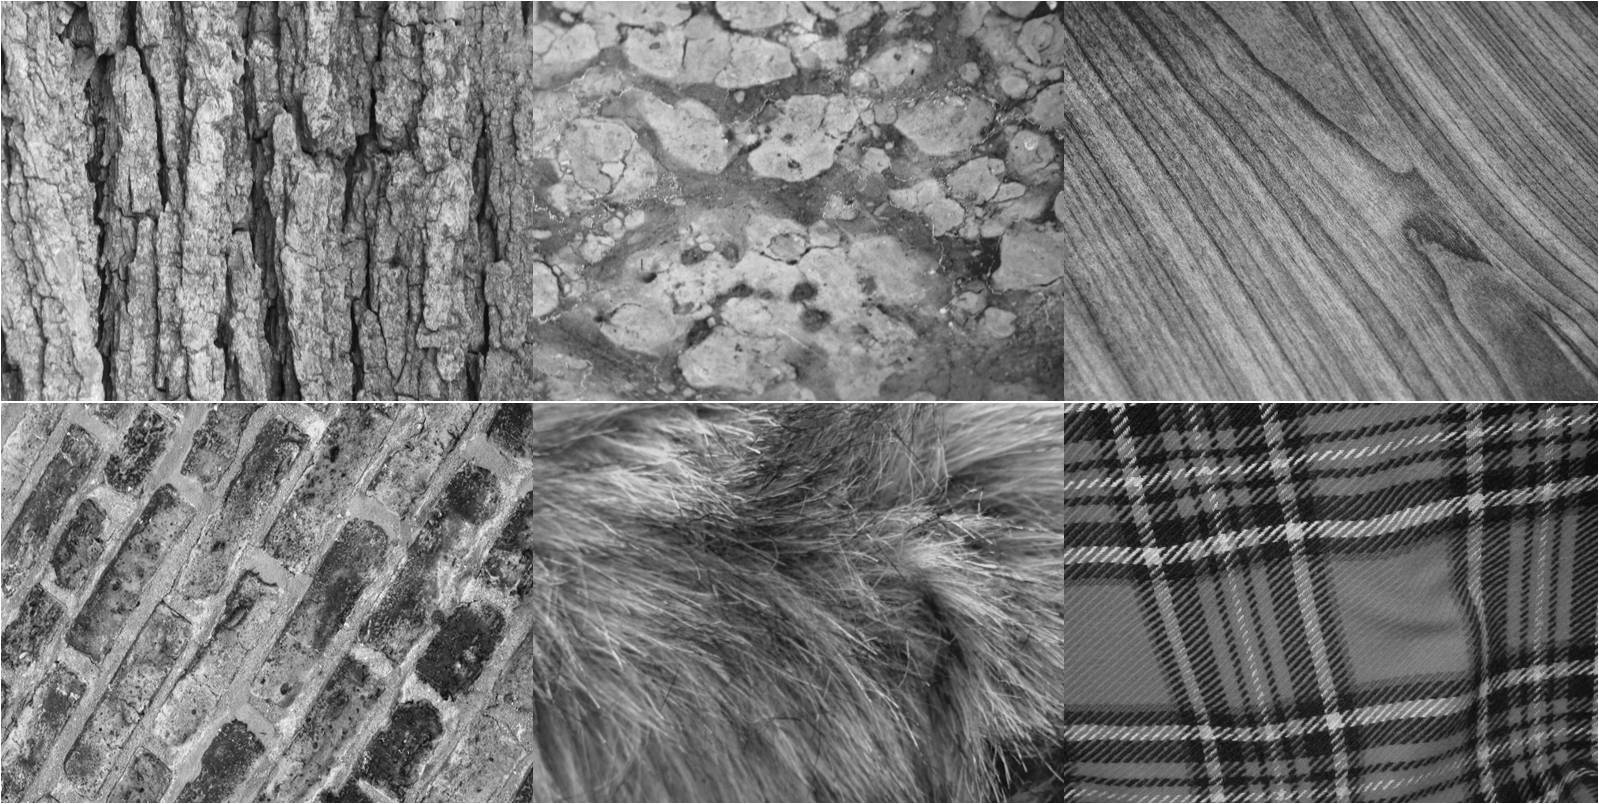
\includegraphics[width=0.4\textwidth]{EjemplosTexturas.jpg}
    \caption{Ejemplos de imágenes de la base de datos}
    \label{fig:ejemplos texturas}
\end{figure}

%------------------------------------------------------------------------
\section{Desarrollo}
Los experimentos realizados con la base de datos mencionada se hicieron representando las imágenes a partir de histogramas de textones. A continuación se detalla cada paso realizado en el desarrollo del trabajo que refleja este documento.

\subsection{Creación del diccionario de textones}
Lo primero que se debe hacer es representar las imágenes en determinado espacio de representación. En este caso se quería trabajar con texturas, por lo que el espacio de representación fue con textones. El uso de textones implica la utilización de varios filtros sencillos y variados en diferentes factores: tamaño (escala), orientación y forma (líneas, barras, círculos). Este método se basa en la idea que un filtro responde en mayor medida en una imagen en los puntos donde se es similar al filtro. De esta manera, lo que se hizo fue tomar una imagen de cada una de las 25 clases y concatenarlas para formar una imagen grande compuesta de una muestra de cada categoría, haciendo que cada clase esté presente en la creación de la librería de textones.

Se filtró esta imagen grande con 32 filtros distintos (como los mencionados anteriormente) y se le asignó a cada píxel qué tanto respondió a cada uno de los filtros. Luego, se realizó un proceso de clustering para agrupar píxeles con respuestas a filtros similares. Para este paso, se varió la cantidad de clusters creados para evaluar el desempeño de los clasificadores según este parámetro. Se crearon representaciones con 5, 10, 15, 20, 25, 30, 35, 40, 45 y 50 clusters de manera independiente. El centroide de cada uno de esos grupos se considera un textón. Por ejemplo, bajo la representación con 20 clusters se crearon 20 vectores (20 centroides), donde cada uno de ellos es un vector de dimensión 32, debido a la respuesta de la imagen sobre los 32 filtros.

Dependiendo la representación en la cantidad de clusters, hay filtros que tienen más o menos peso en los centroides, sin embargo, es posible determinar cuál de todos los filtros discrimina más al evaluar cuál de las 32 dimensiones sobre los centroides tiene mayor varianza. La dimensión de mayor varianza es la del filtro 26 para TODAS las representaciones. Esto quiere decir que los clusters difieren más sobre las respuestas a este filtro que a cualquier otro. Se puede evaluar también el caso contrario hallando la varianza mínima: el filtro que menos discrimina. Al evaluar esto se encuentra que este corresponde al filtro 13 casi siempre, menos en la representación con 30 y 35 clusters, en cuyo caso es el filtro 5.

\begin{figure}[h]
    \centering
    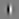
\includegraphics[width=0.1\textwidth]{Filtro26.jpg}
    \caption{Filtro 26. Filtro que más discrimina}
    \label{fig:filtro 26}
\end{figure}

\begin{figure}[h]
    \centering
    
\includegraphics[width=0.07\textwidth]{Filtro13.jpg}
    \caption{Filtro 13. Filtro que menos discrimina}
    \label{fig:filtro 13}
\end{figure}

\subsection{Clasificadores}
Teniendo 10 diferentes representaciones de los textones (varios números de clusters:5, 10, 15, 20, 25, 30, 35, 40, 45 y 50), se procedió a construir un clasificador para reconocer texturas de la base de datos a partir de los textones definidos. 

Se evaluaron dos diferentes tipos de clasificadores: vecino más cercano (Nearest Neighbour) y bosques de decisión (Random Forest):

\subsubsection{Nearest Neighbour (NN)}
El clasificador por vecino más cercano es un clasificador muy sencillo, en el cual, para una imagen de prueba representada de la misma manera que los datos de entrenamiento (mediante textones), se encuentra el cluster que se encuentra más cercano a ese dato.

Lo primero que se hace es que se coge una imagen por cada categoría y se filtra cada píxel con los 32 textones, haciendo que cada píxel tenga un vector de 32 dimensiones asociado, donde cada dimensión corresponde a la respuesta del píxel al filtro correspondiente. Cada píxel es asociado a un cluster de los construidos en la librería de textones (dependiendo de la representación el píxel puede pertenecer a uno entre 5, 10, ..., 45 o 50 clusters), haciendo que ahora cada píxel tenga asociado el número del cluster al que pertenece. Finalmente, se construye un histograma de la imagen a partir de los clusters a los que pertenece cada píxel. De esta manera cada categoría tiene un histograma de textones asociado. Estos 25 histogramas se denominan histogramas de entrenamiento.

Cuando se evalúa una imagen de prueba, esta sigue el proceso mencionado en el párrafo anterior obteniendo un histograma de los textones ahí presentes. Este histograma, cuya cantidad de bins depende de la cantidad de clusters utilizados, es comparado con los 25 histogramas de entrenamiento, hallando con cuál histograma hay mayor semejanza, para asignarle a la imagen de prueba la categoría (de las 25 disponibles) de mayor semejanza. La comparación de histogramas se hace mediante el kernel de intersección, cuya fórmula es: 

\begin{equation}
\cap(H_{1}, H_{2})=\sum_{i}\min{[H_{1}(i),H_{2}(i)]}
\end{equation}
\cite{Interseccion}


Dos histogramas idénticos tendrán intersección de 1, mientras que dos histogramas completamente diferentes tendrán intersección nula.

Se evaluó el desempeño sobre 29 imágenes de validación para encontrar con cuál cantidad de clusters es mejor la clasificación. A partir de este análisis se clasificaron las imágenes de test.

\subsubsection{Random Forest (RF)}
Los RF son grupos de árboles de decisión, donde cada uno decide a cuál categoría pertenece cada dato y se combinan estos scores para llegar a una decisión final sobre el dato evaluado.

Al igual que en NN, lo primero que se hace es construir los histogramas de entrenamiento con imágenes que tienen etiquetas conocidas y asignadas. A diferencia de lo que se hizo con NN, para la construcción de los árboles se variaron dos parámetros: el número de imágenes de entrenamiento (1, 9 y 21, correspondientes al 3.3\%,30\% y 70\% de los datos de entrenamiento, dejando los porcentajes complementarios para la validación) y el número de árboles en el bosque (1, 5, 10, 15, 20, 25 y 30 árboles). Se entrenaron varios bosques variando esos dos parámetros junto con la cantidad de clusters utilizados, obteniendo varios modelos. Se escogió el modelo con menor error de generalización sobre los datos de validación (menor error porcentual sobre predicciones en las imágenes de validación).

Cuando se evalúa una imagen de prueba, se le obtiene su histograma de textones. Este histograma es evaluado por el bosque de decisión, otorgando un score para cada categoría. Al escoger la categoría de mayor score se encuentra la predicción de clase para la imagen de test.
%-------------------------------------------------------------------------
\section{Resultados}
Antes de evaluar resultados sobre imágenes de test es necesario validar el modelo entrenado mediante imágenes de validación. La primera parte de esta sección se enfoca en esa parte, con lo que luego se evalúan las imágenes de test.

\subsection{Nearest Neighbour}
La validación de este clasificador se basaba específicamente en encontrar cuál cantidad de clusters era más adecuada para la clasificación de texturas bajo la base de datos empleada. El error de validación en función del número de clusters se muestra en la figura ~\ref{fig:errorValidacionInterseccion}

\begin{figure}[h]
    \centering
    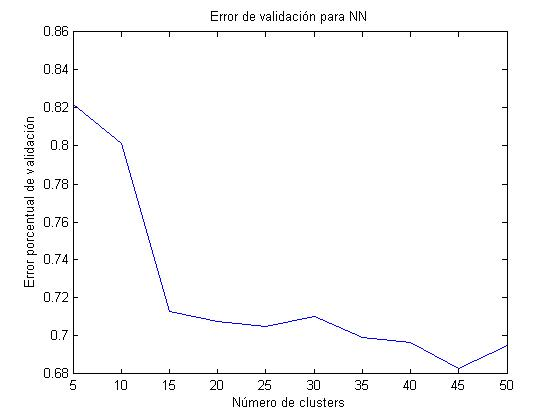
\includegraphics[width=0.5\textwidth]{ErrorValidacionInterseccion.jpg}
    \caption{Error de validación para NN}
    \label{fig:errorValidacionInterseccion}
\end{figure}

Como se puede observar, el mejor modelo es cuando se utilizan 45 clusters, ya que con 50 se observa inicios de overfitting. 

Se construyó también la matriz de confusión para las imágenes de validación bajo este modelo con 45 clusters. Esta matriz se encuentra en la figura ~\ref{fig:ConfusionValidacionInterseccion} e implica un error de clasificación del 68.28\%

\begin{figure}[h]
    \centering
    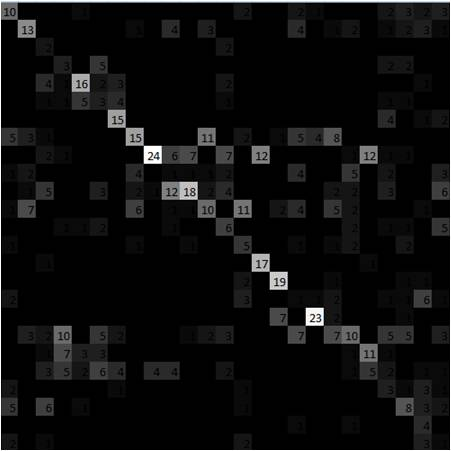
\includegraphics[width=0.3\textwidth]{ConfusionValidacionInterseccion.jpg}
    \caption{Matriz de confusión en la validación de NN con 45 clusters}
    \label{fig:ConfusionValidacionInterseccion}
\end{figure}

Habiendo construido el modelo por Nearest Neighbour con menor error en validación posible según los parámetros intentados, se evaluó el desempeño del clasificador sobre la base de datos de imágenes de test, que correspondía a 10 imágenes por cada una de las 25 categorías (250 imágenes en total). La matriz de confusión de este procedimiento se encuentra en la figura ~\ref{fig:confusionTestInterseccion}, donde se encuentra un error de clasificación del 66.4\%, que como era de esperar, es muy cercano al error obtenido con los datos de validación. Esta similaridad en este valor de sebe a que las imágenes de test y validación/entrenamiento siguen la misma distribución.

\begin{figure}[h]
    \centering
    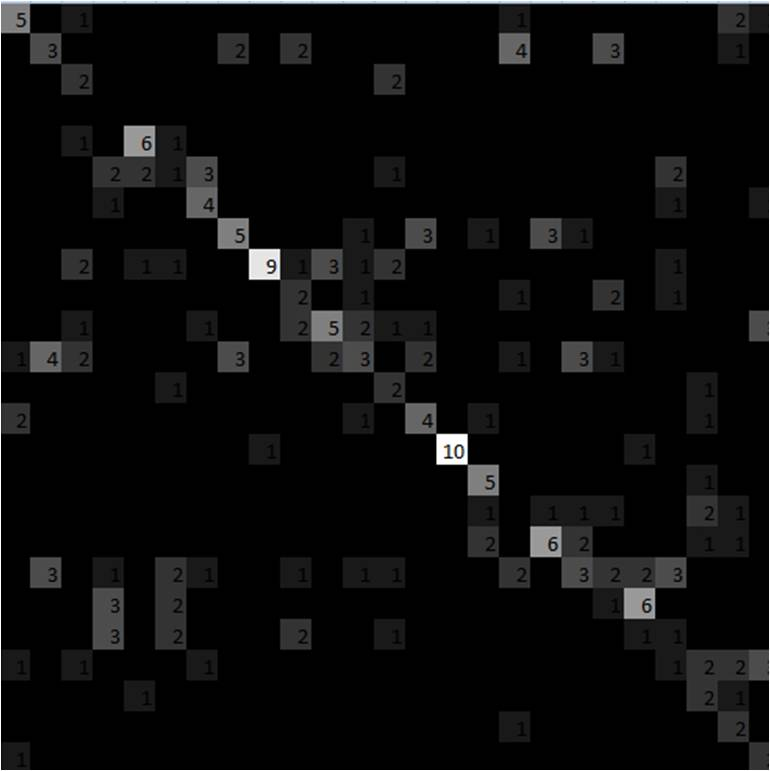
\includegraphics[width=0.3\textwidth]{ConfusionTestInterseccion.jpg}
    \caption{Matriz de confusión en las imágenes de test clasificadas con NN (kernel intersección) con 45 textones}
    \label{fig:confusionTestInterseccion}
\end{figure}

\subsection{Random Forest}
La validación de este clasificador tuvo en cuenta más parámetros: cantidad de clusters, número de árboles y número de imágenes de entrenamiento. Se realizó el entrenamiento del modelo variando estos parámetros y encontrando el error promedio de clasificación sobre los datos de validación. El resultado de este paso se encuentra en las figuras ~\ref{fig:errorValidacion1} (para 1 imagen de entrenamiento), ~\ref{fig:errorValidacion9} (para 9 imágenes de entrenamiento) y  ~\ref{fig:errorValidacion21} (para 21 imágenes de entrenamiento).

\begin{figure}[h]
    \centering
    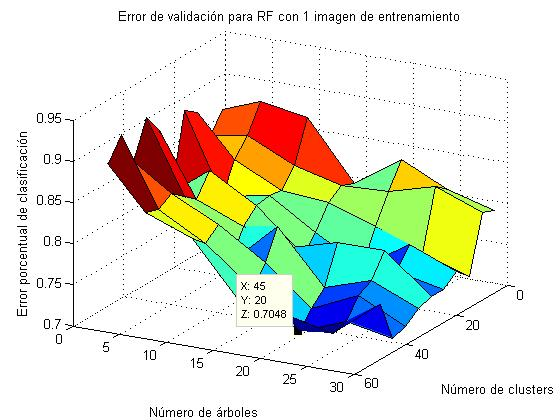
\includegraphics[width=0.5\textwidth]{ErrorValidacion1.jpg}
    \caption{Error de validación para RF con 1 imagen de entrenamiento}
    \label{fig:errorValidacion1}
\end{figure}

\begin{figure}[h]
    \centering
    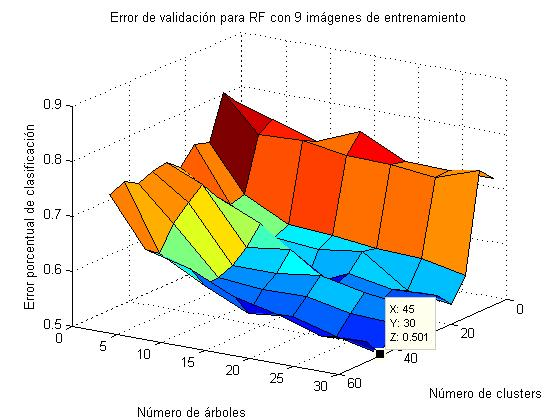
\includegraphics[width=0.5\textwidth]{ErrorValidacion9.jpg}
    \caption{Error de validación para RF con 9 imágenes de entrenamiento}
    \label{fig:errorValidacion9}
\end{figure}

\begin{figure}[h]
    \centering
    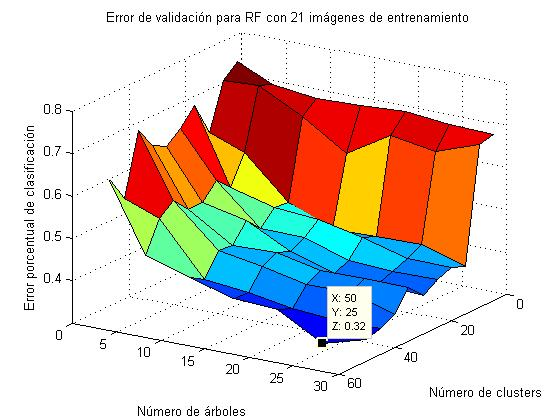
\includegraphics[width=0.5\textwidth]{ErrorValidacion21.jpg}
    \caption{Error de validación para RF con 21 imágenes de entrenamiento}
    \label{fig:errorValidacion21}
\end{figure}

Se encontró, entonces, que el mejor modelo es con 21 imágenes de entrenamiento, 25 árboles y 50 clusters, ya que este modelo entregó el menor error de clasificación sobre los datos de validación (32\%). Este mismo modelo mostró un error sobre los datos de entrenamiento del 0\%. Se construyó también la matriz de confusión para las imágenes de validación y entrenamiento bajo este mejor modelo. Estas matrices se encuentran en las figuras ~\ref{fig:ConfusionValidacionRF} y ~\ref{fig:ConfusionEntrenamientoRF} e implican un error de clasificación del 32\% y 0\% correspondientemente

\begin{figure}[h]
    \centering
    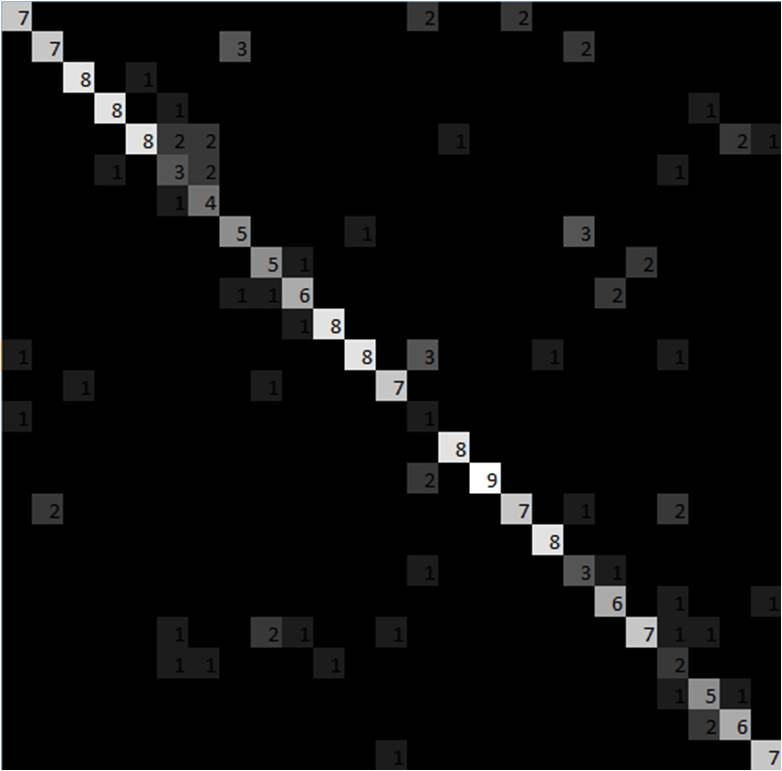
\includegraphics[width=0.3\textwidth]{ConfusionValidacionRF.jpg}
    \caption{Matriz de confusión en la validación de RF con 21 datos de entrenamiento, 25 árboles y 50 clusters}
    \label{fig:ConfusionValidacionRF}
\end{figure}

\begin{figure}[h]
    \centering
    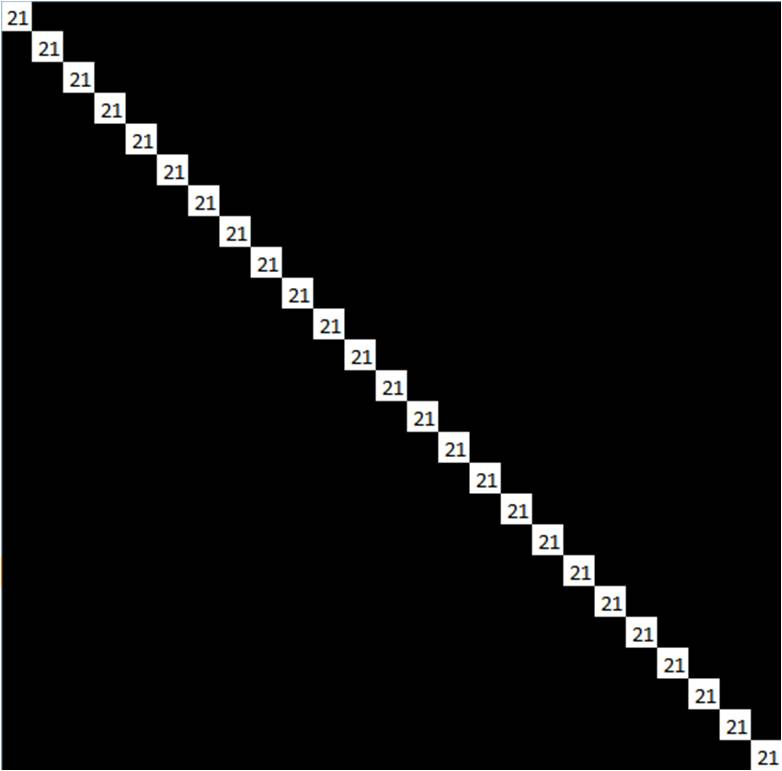
\includegraphics[width=0.3\textwidth]{ConfusionEntrenamientoRF.jpg}
    \caption{Matriz de confusión en el entrenamiento de RF con 21 datos de entrenamiento, 25 árboles y 50 clusters}
    \label{fig:ConfusionEntrenamientoRF}
\end{figure}

Habiendo construido el modelo por Random Forest con menor error en validación posible según los parámetros intentados (21 imágenes de entrenamiento, 25 árboles y 50 textones), se evaluó el desempeño del clasificador sobre la base de datos de imágenes de test, que correspondía a 10 imágenes por cada una de las 25 categorías (250 imágenes en total). La matriz de confusión de este procedimiento se encuentra en la figura ~\ref{fig:confusionTestRF}, donde se encuentra un error de clasificación del 37\%, que como era de esperar, es muy cercano al error obtenido con los datos de validación. Esta similaridad en este valor de sebe a que las imágenes de test y validación/entrenamiento siguen la misma distribución.

\begin{figure}[h]
    \centering
    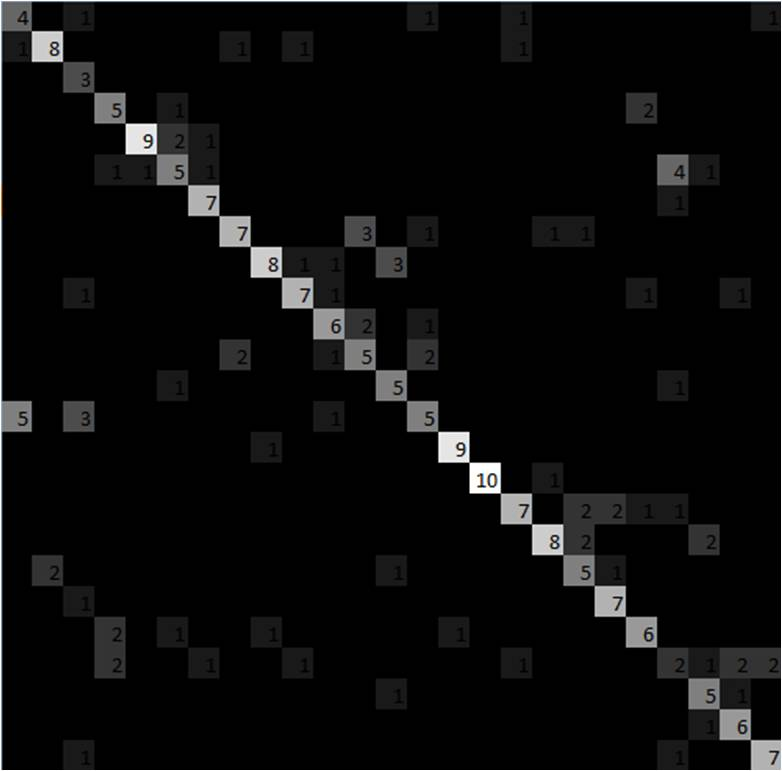
\includegraphics[width=0.3\textwidth]{ConfusionTestRF.jpg}
    \caption{Matriz de confusión en las imágenes de test clasificadas con Random Forest con 50 textones, 25 árboles y 70\% de imágenes de entrenamiento}
    \label{fig:confusionTestRF}
\end{figure}
%-------------------------------------------------------------------------
\section{Discusión}
Luego de construir dos clasificadores distintos sobre la misma base da datos para realizar clasificación de texturas y evaluar el desempeño de cada uno mediante la matriz de confusión y el error porcentual de clasificación, es posible realizar una comparación más detallada de los mismos.

Para el caso del clasificador mediante Nearest Neighbour con kernel de intersección, el mejor modelo fue el construido con 45 textones; mientras que usando Random Forest, el mejor modelo es el de 45 árboles, 50 textones y entrenado con 21 imágenes de entrenamiento.Es claro, tanto por la matriz de confusión como por el error calculado, que el clasificador mediante Random Forest funciona mejor, teniendo más aciertos en la clasificación de imágenes según la textura. 

Al analizar las matrices de confusión, se puede evidenciar que hay trs categorías que causan bastante confusión: la 1, la 3 y la 22, ya que en las matrices de confusión, el valor de la diagonal para cada una de estas clases es muy bajo. Esto significa que los clasificadores construidos tienen problemas identificando estas tres categorías, confundiendolas con otras. A diferencia de estas tres, las clases 5, 15 y 16 son las de menor confusión mediante los algoritmos construidos.

Otra manera de evaluar el desempeño de los clasificadores es mediante el tiempo que emplea cada uno en el entrenamiento, validación y evaluación. Los tiempos de ejecución de diferentes pasos de este experimento se muestran a continuación:

La generación de histogramas de textones (para las 10 diferentes cantidades de clusters probados) para las 750 imágenes de entrenamiento y validación tomó 16837 segundos (unas 4.7 horas). Para Nearest Neighbour no hay un proceso de entrenamiento explícito, por lo que ese es el tiempo de entrenamiento. En Random Forest se requiere un entrenamiento de los árboles de decisión, por lo que esas 4.7 horas deben ser sumadas a los siguientes tiempos:

\begin{table}[h]
\centering
\begin{tabular}{ll}
\multicolumn{2}{c}{Entrenamiento Random Forest} \\ \hline
\multicolumn{1}{|l|}{Imágenes de entrenamiento por clase} & \multicolumn{1}{l|}{Tiempo (s)} \\ \hline
\multicolumn{1}{|l|}{1} & \multicolumn{1}{l|}{26,2} \\ \hline
\multicolumn{1}{|l|}{9} & \multicolumn{1}{l|}{73,6} \\ \hline
\multicolumn{1}{|l|}{21} & \multicolumn{1}{l|}{133,5} \\ \hline
\end{tabular}
\caption{Tiempos de entrenamiento para Random Forest}
\label{table: tiemposEntrenamientoRF}
\end{table}

Para la validación de los modelos, es decir, para encontrar la combinación de parámetros de mejor desempeño, se encontró el error de clasificación para cada combinación de parámetros intentada. Los tiempos de este paso (sobre las imágenes de validación) fueron los siguientes:

\begin{table}[h]
\centering
\begin{tabular}{|l|l|}
\hline
Número de imágenes de entrenamiento & Tiempo (s) \\ \hline
1 & 7,33 \\ \hline
9 & 6,44 \\ \hline
21 & 2,75 \\ \hline
Nearest Neighbour & 33,32 \\ \hline
\end{tabular}
\caption{Tiempos para cálculo del error sobre validación}
\label{table: tiemposError}
\end{table}

El tiempo para el entrenamiento del modelo final del Random Forest (21 imágenes de entrenamiento, 25 árboles y 50 textones) fue de 4,44 segundos.

Finalmente, el tiempo de evaluación para una imagen de prueba es sumamente importante, ya que un clasificador que se demore mucho tiempo evaluado una imagen no es eficiente, por más que el error de clasificación sea muy bajo. La comparación del tiempo de evaluación sobre las 250 imágenes de prueba para los dos modelos se muestra en las tablas ~\ref{table: tiemposRepresentacion} y ~\ref{table: tiemposEvaluacion}, donde la primera corresponde al tiempo para representar cada imagen como histograma de textones y la segunda al tiempo para clasificar cada imagen. La diferencia en los tiempos en la tabla ~\ref{table: tiemposRepresentacion} se debe a que el modelo de Nearest Neighbour requiere un histograma con 45 bins, mientras que el clasificador por Random Forest lo requiere con 50 bins.

\begin{table}[h]
\centering
\begin{tabular}{|l|l|}
\hline
Clasificador & \begin{tabular}[c]{@{}l@{}}Tiempo para representación\\ aprox. por imagen \end{tabular} \\ \hline
Nearest Neighbour & 2,38 s \\ \hline
Random Forest & 2,94 s \\ \hline
\end{tabular}
\caption{Tiempos para representar cada imagen como historama de textones según lo necesitado por el clasificador}
\label{table: tiemposRepresentacion}
\end{table}

\begin{table}[h]
\centering
\begin{tabular}{|l|l|}
\hline
Clasificador & \begin{tabular}[c]{@{}l@{}}Tiempo de evaluación\\ aprox. por imagen \end{tabular} \\ \hline
Nearest Neighbour & 2,36 ms \\ \hline
Random Forest & 1,44ms \\ \hline
\end{tabular}
\caption{Tiempos de evaluación}
\label{table: tiemposEvaluacion}
\end{table}

Se puede observar que el tiempo de evaluación es muy similar para los dos clasificadores, siendo un poco menor para NN, ya que este utiliza vectores de menor dimensión. Teniendo en cuenta que los tiempos de evaluación son muy similares pero RF tiene un error del 37\% frente al 66,4\% de error logrado con NN, se concluye que el clasificador por Random Forest construido tiene un mejor desempeño sobre la base de datos utilizada para clasificación de imágenes según sus textones
%-------------------------------------------------------------------------
\section{Conclusiones, limitaciones y mejoras potenciales}
Se construyeron dos clasificadores para abordar el problema de clasificación de imágenes según sus texturas: Nearest Neighbour con kernel de intersección (NN) y Random Forest (RF). Cada uno de los métodos fue entrenado y validado variando diferentes parámetros: cantidad de textones para NN; cantidad de textones, número de árboles y número de imágenes de entrenamiento para RF. Al calcular el error de clasificación sobre las imágenes de validación, fue posible escoger la mejor combinación de parámetros para los dos modelos con sus respectivos errores sobre validación:
\begin{itemize}
\item NN: 45 textones. Error del 68.28\% sobre validación.
\item RF: 50 textones, 25 árboles y 70\% de datos de entrenamiento (21 imágenes). Error del 32\% sobre validación.
\end{itemize}

Se evaluaron 250 imágenes de prueba con los dos clasificadores escogidos obteniendo que el mejor modelo es el de Random Forest con un 37\% de error, contra el modelo de Nearest Neighbour que obtuvo un 66,4\% de error sobre dichas imágenes. La comparación de tiempos de evaluación por imagen mostró que los dos modelos toman casi el mismo tiempo (entre 2 y 3 segundos por imagen), siendo NN ligeramente más rápido en representación debido a que las imágenes son representadas con menos dimensiones que en RF. En evaluación RF es claramente más rápido por imagen.

Se concluye que el mejor clasificador de los dos construidos es el de Random Forest con 50 textones, 25 árboles y entrenado con 21 imágenes. Aún así, el desempeño no es el mejor, ya que un error cercano al 30\% no es el deseado. Para mejorar el desempeño y bajar el error de clasificación se puede mejorar el método de diversas formas:
\begin{itemize}
\item Aumento del número de imágenes por categoría, ya que de esta manera habrían más imágenes disponibles para entrenar al modelo.
\item Evaluación del modelo con un mayor número de textones o árboles. Esto no se pudo hacer exhaustivamente por limitaciones de memoria computacional.
\item Variación del número de nodos de los árboles, es decir, modulación del \textit{prunning} sobre cada uno de ellos.
\item Se podría evaluar el desempeño de otros tipos de clasificadores, como por ejemplo SVM.
\item Se podría añadir información de color a las imágenes, ya que el color también puede afectar de manera importante a las texturas.
\end{itemize}

Aparte de esto, la base de datos tiene algunas limitaciones, como por ejemplo el ya mencionado número de imágenes de entrenamiento. Tener únicamente 30 imágenes por categoría para entrenar un clasificador multiclase con 25 categorías no es óptimo. Sería ideal tener un número mucho mayor de imágenes de entrenamiento por categoría para lograr construir clasificadores con mejor desempeño. Otra limitación del la base de datos es que hay únicamente 25 clases. Si se evalúa una imagen con textura diferente a las 25 categorías, el modelo no va a ser capaz de predecir su verdadera textura, sino que la va a tomar como una de las 25 texturas de la base de datos. 


%-------------------------------------------------------------------------

{\small
\bibliographystyle{plain}
\bibliography{bibliografia}{}
}

\end{document}